\documentclass[11pt]{article}
\usepackage{icmlko}
\begin{document}

\title{판 안에도 옆방이 있었다 --- 학습 문턱 40 은 팝업을 안 본 도메인으로 만들고 있었다}
\author{월드모델 실험실}
\date{노트 402 · 2026년 8월 1일}
\maketitle

\begin{abstract}
노트 398부터 401까지 네 노트가 \emph{안 본 도메인}의 값을 쟀다 --- 학습에
없는 도메인은 F18 에게 원핫이 전부 0 인 좌표를 받고, 그 좌표에서 KR 만화는
$-0.1261$ 로 \textbf{거꾸로} 줄을 선다. 그동안 그것을 판 \emph{바깥}
이야기로 다뤘다. \textbf{판 안에 이미 하나 있었다.}

학습 문턱(\texttt{MIN\_TRAIN})은 \textbf{학습만} 거른다 --- 문턱 아래
도메인은 훈련 집합에서 빠지고도 \textbf{채점은 그대로 받는다}. 팝업의 학습
행은 \textbf{24행}이다. 커밋된 기본값 40 에서 팝업은 \textbf{배우지 않은
채로 채점되는 도메인}, 곧 원핫이 전부 0 인 바로 그 좌표에 서 있었다.

\begin{center}
\begin{tabular}{lrrr}
\hline
짝 12뽑기, 문턱 40 $-$ 문턱 15 & 차 & SD & 부호 \\
\hline
\textbf{판} & $\mathbf{-0.0018}$ & $0.0021$ & $\mathbf{2/12}$ \\
\hline
\textbf{팝업} (학습 24행) & $\mathbf{-0.0525}$ & $0.0254$ & $1/12$ \\
도서 (다음으로 큰 것) & $-0.0083$ & $0.0084$ & $2/12$ \\
나머지 아홉 & $|{\cdot}| \le 0.0034$ & --- & --- \\
\hline
\end{tabular}
\end{center}

사전 등록대로다 --- \textbf{움직인 도메인은 팝업 하나뿐}이고 나머지 열은
잡음 안이다. 두 팔이 \textbf{같은 열한 도메인}을 채점하므로(문턱은 학습만
거른다) 노트 378 ④ 에 걸리지 않고 잴 수 있다. 판 차가 $2\times$짝SD 안이고
부호가 $2/12 \le 3/12$ 라 조건 ① 이 걸린다 --- \textbf{문턱 15 를 채택}했다.
\end{abstract}

\section{같은 기계, 판 안에서}

노트 399가 원핫을 통째로 빼서 KR 만화의 전이를 $-0.1261 \to +0.0797$ 로
$0.2058$ 만큼 움직였다. 문턱을 40 에서 15 로 내려 팝업을 학습에 들이면
$0.0525$ 가 움직인다. 크기는 4분의 1이지만 \textbf{기계가 같다} --- 둘 다
``원핫이 전부 0 인 좌표에 세워 두면 얼마나 손해인가''를 잰다.

크기가 작은 것도 설명이 된다. KR 만화는 학습에 \emph{한 행도} 없었지만,
문턱 40 의 팝업은 채점만 안 배운 게 아니라 \textbf{자기 24행이 다른 도메인의
축 모형에 보태지지도} 못했다 --- 대신 팝업의 유보 행은 아이돌·시장팝업 같은
이웃 도메인이 만든 축 지도를 빌려 쓴다. 완전한 이방인은 아니었다.

\section{왜 이걸 이제야 쟀나}

문턱은 2년째 40이었고 그 값이 무엇을 하는지 적혀 있지 않았다. 노트 401이
\textbf{조용한 탈락}에 관한 규약을 만든 직후에야 보였다 --- \emph{도메인을
거르는 집계 문턱은 전부 누가 빠졌는지 찍고 지나간다.} 401에서는 반례
도메인이 상관 계산에서 빠졌고, 여기서는 같은 도메인이 \textbf{학습에서}
빠져 있었다. 같은 팝업이다.

노트 401의 셈에서 팝업의 학습 24행이 잡음 바닥($0.221$)보다 작은 어긋남
($0.179$)을 냈던 것도 이제 다르게 읽힌다 --- 그 24행은 \textbf{그때까지
챔피언이 한 번도 안 본 행}이었다.

\section{남은 것}

\begin{tabular}{lp{7.4cm}}
\hline
원핫을 크기로 거른다 & 팝업은 드롭아웃엔 \textbf{벌고}($+0.0276 \cdot 12/12$,
노트 400) 문턱 40 엔 \textbf{잃는다}($-0.0525$). 제 행은 원하고 제 원핫은
원치 않는다 --- 큰 도메인만 원핫을 주면 둘 다 갖나 \\
문턱 15 아래 & 15 도 근거 없는 값이다. 팝업 24행이 유일한 걸림이었으니 더
내려도 지금은 아무것도 안 바뀐다 \\
다른 조용한 문턱 & 가드·집계·수집에 같은 종류가 더 있나 \\
\hline
\end{tabular}

\begin{figure}[h]
\centering
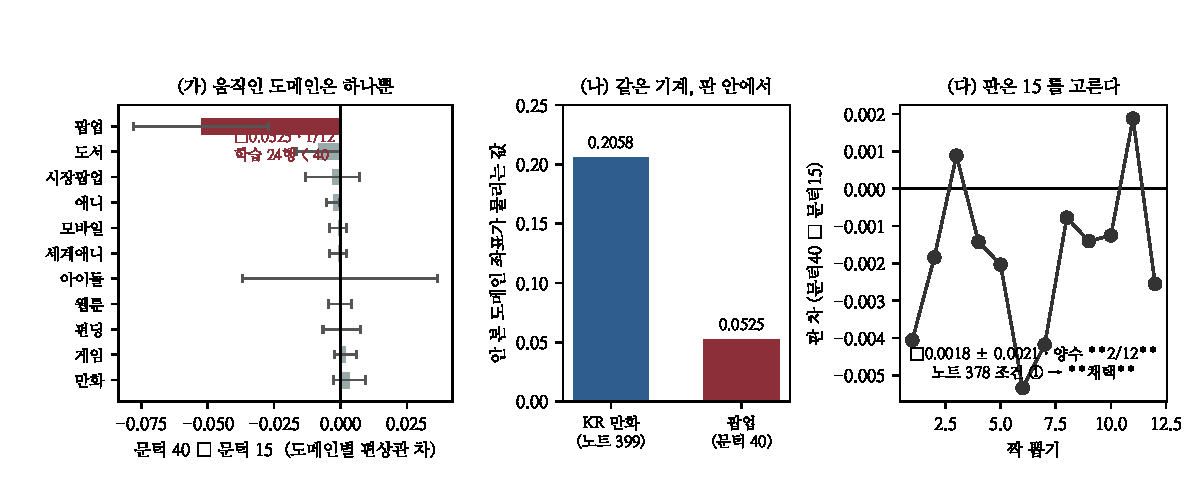
\includegraphics[width=\textwidth]{figs/fig402.pdf}
\caption{(가) 문턱 40 은 팝업에서만 물린다 --- 나머지 열은 잡음 안. 막대는
짝 12뽑기 평균, 수염은 SD. (나) 같은 기계의 두 눈금 --- KR 만화(학습에
한 행도 없음)와 팝업(문턱 아래). (다) 판 차는 열두 뽑기 중 열에서 음수다.}
\end{figure}

\end{document}
